\chapter{Синтез линейных непрерывных систем}
\setcounter{section}{8} %TODO:Remove
\setcounter{subsection}{2} %TODO:Remove
\setcounter{equation}{23} %TODO:Remove
\setcounter{figure}{7}%TODO:Remove

\subsection{Идентификационное каноническое представление системы с одним (скалярным) выходом}
С помощью рассуждений, аналогичных проведённым в п.3.8.1, можно получить следующие результаты.

Если пара матриц    полностью наблюдаема,  то  в   пространстве состояний  Х  всегда существует базис, в котором пара ${A,C}$  имеет идентификационное каноническое представление (ИКП):
\begin{equation}
	A_I = 
	\begin{bmatrix}
	    0 & 0 & \dots & 0 & 0 & -\alpha_n \\
	    1 & 0 & \dots & 0 & 0 & -\alpha_{n-1} \\
	    0 & 1 & \dots & 0 & 0 & -\alpha_{n-2} \\
	    \dots & \dots & \dots & \dots & \dots & \dots \\
	    0 & 0 & \dots & 0 & 0 & -\alpha_3 \\
	    0 & 0 & \dots & 1 & 0 & -\alpha_2 \\
	    0 & 0 & \dots & 0 & 1 & -\alpha_1
	\end{bmatrix}
\end{equation}

\begin{equation}
	C_I = 
	\begin{bmatrix}
	    0 & 0 & \dots & 0 & 0 & 1
	\end{bmatrix}
\end{equation}

Отметим, что

\begin{equation}
	A_I^T = A_U; C_I^T=\vec{b}_U.
\end{equation}

Если   в  некотором  исходном  базисе [$h$] заданы матрицы $A_H, C_H$ и если система полностью наблюдаема, то, для того чтобы вычислить их (матриц) ИКП, достаточно вычислить коэффициенты характеристичес¬кого полинома $\phi_A(\lambda)$ . После этого может быть вычислена матрица преобразования от исходного базиса [$h$] к ИКП в соответствии с (3.7.13):

\begin{equation}
	I_H^{-1}=N_I^{-1}N_H.
\end{equation}

Если известна матрица $B_H$ при векторе управления в исходном базисе, то с учётом (3.6.8)  в базисе ИКП она может быть определена с помощью соотношения

\begin{equation}
	B_I=I_H^{-1}B_H
\end{equation}

\subsection{Передаточная функция и структура для системы в ИКП}
В соответствии с видом матриц $A_I$ и $C_I$ уравнения системы со скалярным входом $u$ и скалярным выходом $y$  имеют вид

\begin{equation}
\begin{cases}
	\dot{x}_{i1} = -\alpha_nx_{in}+b_{i1}u;\\
	\dot{x}_{i2} = x_{i1} - \alpha_{n-1}x_{in}+b_{i2}u;\\
	\dot{x}_{i3} = x_{i2} - \alpha_{n-2}x_{in}+b_{i3}u;\\
	\begin{tabular}{ l l l l l l }
	  \dots & \dots & \dots & \dots & \dots & \dots 
	\end{tabular}
	\dot{x}_{in-1} = x_{in-2} - \alpha_{2}x_{in}+b_{in-1}u;\\
	\dot{x}_{in} = x_{in-1} - \alpha_{1}x_{in}+b_{in}u;\\
\end{cases}
\end{equation}

\begin{equation}
	y = x_{in}
\end{equation}

Этим уравнениям соответствует структурная схема, представленная на рис. 3.8.

\begin{figure}[H]
	\centering
	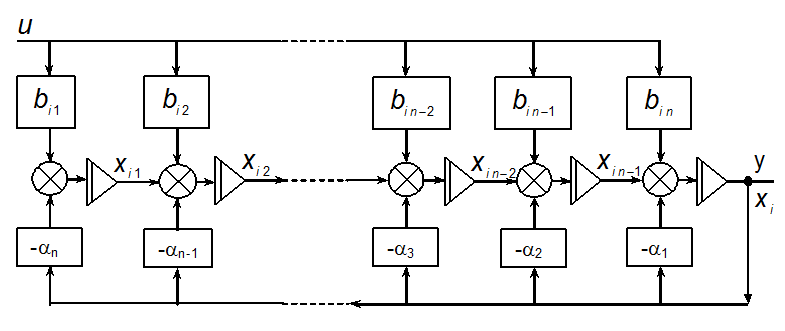
\includegraphics[scale=0.9]{images/Fig3_8}
	\caption{Схема моделирования системы в ИКП}
\end{figure}

В соответствии с этим рисунком передаточная функция системы имеет вид

\begin{multline}
	W_{u,y}(p) = \dfrac{b_{i1}p^{-n}+b_{i2}p^{-(n-1)}+\dots+b_{in-1}p^{-2}+b_{in}p^{-1}}{1+\alpha_1p^{-1}+\alpha_2p^{-2}+\dots+\alpha_np^{-n}} = \\
	\dfrac{b_{i1}+b_{i2}p+\dots+b_{in-1}p^{n-2}+b_{in}p^{n-1}}{p^n+\alpha_1p^{n-1}+\alpha_2p^{n-2}+\dots+\alpha_{n-1}p+\alpha_n}.
\end{multline}

Отметим, что статический передаточный коэффициент

\begin{equation}
	W_{u,y}(0)=\dfrac{b_{i1}}{\alpha_n}
\end{equation}

\newpage

\section{Обратная связь по состоянию, обеспечивающая заданное (желаемое) расположение собственных чисел в замкнутой системе с одним (скалярным) входом}

Даны уравнения полностью управляемого объекта управления в некотором исходном базисе

\begin{gather}
\begin{split}
	\dot{\vec{x}}_H(t) = A_H\vec{x}_H(t)+\vec{b}_Hu(t);\\
	y(t)=C_H\vec{x}_H(t),
\end{split}
\end{gather}
каждая координата вектора состояния которого доступна для измерения.
Требуется синтезировать такое управление, которое бы обеспечило требуемое качество отработки внешнего командного сигнала $v(t)$.

Динамические свойства системы управления в основном определяются её собственными числами, то есть нулями характеристического полинома
\begin{equation}
	\phi_A(\lambda) = \prod_{i=1}^{n}(\lambda - \lambda_i)=\lambda^n+\alpha_1\lambda^{n-1}+\dots+\alpha_n.
\end{equation}

Время переходного процесса каждой моды определяется расстоянием до мнимой оси вещественной части; колебательность - соотношением мнимой и вещественной частей соответствующих собственных чисел. Эти зависимости могут быть проанализированы при изучении характеристик типовых звеньев, кроме того, они рассматриваются в обширной учебной литературе по теории автоматического регулиро-вания и управления.

В соответствии со структурной схемой, приведённой на рис. 3.9, сформируем сигнал управления объектом в виде
\begin{equation}
	u(t) = L_H\vec{x}_H(t) + k^vv(t)
\end{equation}
где $L_H$ – некоторая матрица-строка обратной связи:
\begin{equation}
	L_H = [\begin{tabular}{ l l l l }
		  	$l_{h1}$ & $l_{h2}$ & $\dots$ & $l_{hn}$
		  \end{tabular}]
\end{equation}
$k^v$ – коэффициент по командному сигналу.
Тогда уравнение системы примет вид
\begin{equation}
	\dot{\vec{x}}_H(t)=A_H\vec{x}_H(t)+\vec{b}_HL_H\vec{x}_H(t)+\vec{b}_Hk^vv(t),
\end{equation}
или
\begin{equation}
	\dot{\vec{x}}_H(t)=A_H^C\vec{x}_H(t)+\vec{b}_Hk^vv(t),
\end{equation}
где $A_H^C$ - матрица замкнутой системы в исходном базисе:
\begin{equation}
	A_H^C=A_H+\vec{b}_HL_H
\end{equation}

\begin{figure}[H]
	\centering
	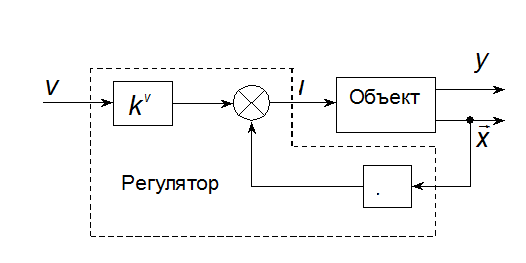
\includegraphics[scale=0.9]{images/Fig3_9}
	\caption{Структурная схема замкнутой системы}
\end{figure}

Поскольку объект полностью управляем, то существует базис [$u$], в котором пара $\{A,\vec{b}\}$ имеет управляемое каноническое представление $\{A_U,\vec{b}_U\}$ . Поэтому перейдём к записи уравнений системы в базисе УКП. В соответствии с (3.4.16) произведём замену 
\begin{equation}
	\vec{x}_H=U_H\vec{x}_U
\end{equation}
Тогда из (3.9.1) получим
\begin{equation}
	U_H\dot{\vec{x}}_U(t)=A_HU_H\vec{x}_U(t)+\vec{b}_Hu(t);
\end{equation}
\begin{equation}
	y(t)=C_HU_H\vec{x}_U.
\end{equation}
Умножив уравнение (3.9.9) слева на $U_H^{-1}$, будем иметь
\begin{gather}
\begin{split}
	\dot{\vec{x}}_U(t)=A_U\vec{x}_U(t)+\vec{b}_Uu(t);\\
	y(t) = C_U\vec{x}_U(t),
\end{split}
\end{gather}
где $A_U$ $\vec{b}_U$ и $C_U$ - соответствующие матрицы в УКП.

Используя подстановку (3.9.8), из (3.9.3) получим
\begin{equation}
	u(t)=L_U\vec{x}_U+k^vv(t),
\end{equation}
где матрица обратной связи в базисе УКП
\begin{equation}
	L_U=L_HU_H.
\end{equation}

В результате  уравнение замкнутой системы  в базисе управляемого канонического представле¬ния будет иметь вид
\begin{equation}
	\dot{\vec{x}}_U(t)=A_U^C\vec{x}_U(t)+\vec{b}_U \cdot k^vv(t)
\end{equation}
Здесь $A_U^C$ является сопровождающей матрицей по отношению к характеристическому полиному замкнутой системы
\begin{equation}
	\phi_{A^C}(\lambda) - \prod_{i=1}^{n}(\lambda - \lambda_i^3)=\lambda^n+\gamma_1\lambda^{n-1}+\dots+\gamma_n,
\end{equation}
поэтому она имеет стандартный вид
\begin{equation}
	A_U^C = 
	\begin{bmatrix}
	    0 & 1 & 0 & \dots & 0 \\
	    0 & 0 & 1 & \dots & 0 \\
	    \dots & \dots & \dots & \dots & \dots \\
	    0 & 0 & 0 & \dots & 1 \\
	    -\gamma_n &  -\gamma_{n-1} & -\gamma_{n-2} & \dots & -\gamma_1 \\
	\end{bmatrix}
\end{equation}
С другой стороны, очевидно, что
\begin{equation}
	A_U^C=A_U+\vec{b}_UL_U.
\end{equation}
Отсюда сразу же следует связь между коэффициентами характеристического полинома (3.9.2) объекта и коэффициентами характеристического полинома (3.9.14) желаемой системы:
\begin{equation}
	-\gamma_i=-\alpha_i+l_{Un-i+1}, i=1,2,\dots,n.
\end{equation}
Далее обусловлены следующие действия.
\begin{enumerate}
\renewcommand\labelenumi{\theenumi.}
\item Задание желаемых собственных чисел замкнутой системы $\lambda_1^3,\lambda_2^3,\dots,\lambda_n^3,$
\item Вычисление коэффициентов характеристического полинома замкнутой системы $\gamma_1,\gamma_2,\dots,\gamma_n$ в соответствии с выражением (3.9.15).
\item 3.	Вычисление согласно (3.9.17) коэффициентов матрицы обратной связи в базисе УКП:
\begin{equation}
	l_{U,n-i+1}=\alpha_i-\gamma_i, i=1,2,\dots,n.
\end{equation}
\item Вычисление в соответствии с (3.9.12) и (3.8.17) матрицы обратной связи в исходном базисе:
\begin{equation}
	L_H=L_UU_UU_H^{-1}.
\end{equation}
\item Определение величины коэффициента $k^v$ в соответствии с требованиями по статике.
\end{enumerate}

Так, например, если требуется обеспечить единичную статику по командному сигналу $v$, то это значит, что установившееся значение переходной функции $h(t)$ замкнутой системы должно быть равно единице. Одним из свойств передаточной функции устойчивой системы является равенство
\begin{equation}
	\lim\limits_{t\to\infty}h(t)=\lim\limits_{p\to0}W_{vy}(p)
\end{equation}
Согласно структурной схеме, приведённой на  рис. 3.9, передаточная функция между командным $v$ и выходным $y$ сигналами имеет вид
\begin{equation}
	W_{vy}(p)=k^v\cdot W(p)
\end{equation}
где передаточная функция $W(p)$ может быть определена аналогично выражению (3.8.22). Таким образом, получаем
\begin{equation}
	h(\infty)=k^v\dfrac{c_{U1}}{\gamma_n}=1,
\end{equation}
откуда, окончательно,
\begin{equation}
	k^v=\dfrac{\gamma_n}{c_U1}
\end{equation}
\newpage